\subsection{Architettura backend}

\subsubsection{Descrizione generale} 
L’architettura del backend adotta lo stile modulare fornito da NestJS, basandosi su una suddivisione in moduli indipendenti, ciascuno responsabile di una specifica funzionalità dell’applicazione. Ogni modulo è organizzato secondo un approccio a layer, comprendente controller, servizi e provider.\\
Il ruolo principale del backend è quello di fungere da mediatore tra diverse fonti di dati esterne (principalmente API REST), aggregando e trasformando le informazioni ricevute in un formato uniforme e coerente. I dati vengono quindi resi disponibili tramite endpoint REST standardizzati. Le sorgenti dati sono gestite da componenti chiamati \textit{fetcher}, ciascuno progettato per interagire con un'API specifica. Tutti i \textit{fetcher} seguono la stessa interfaccia, il che rende facile aggiungere nuove fonti di dati in futuro.

\subsubsection{Diagramma delle classi}
\begin{figure}[H]
    \begin{center}
        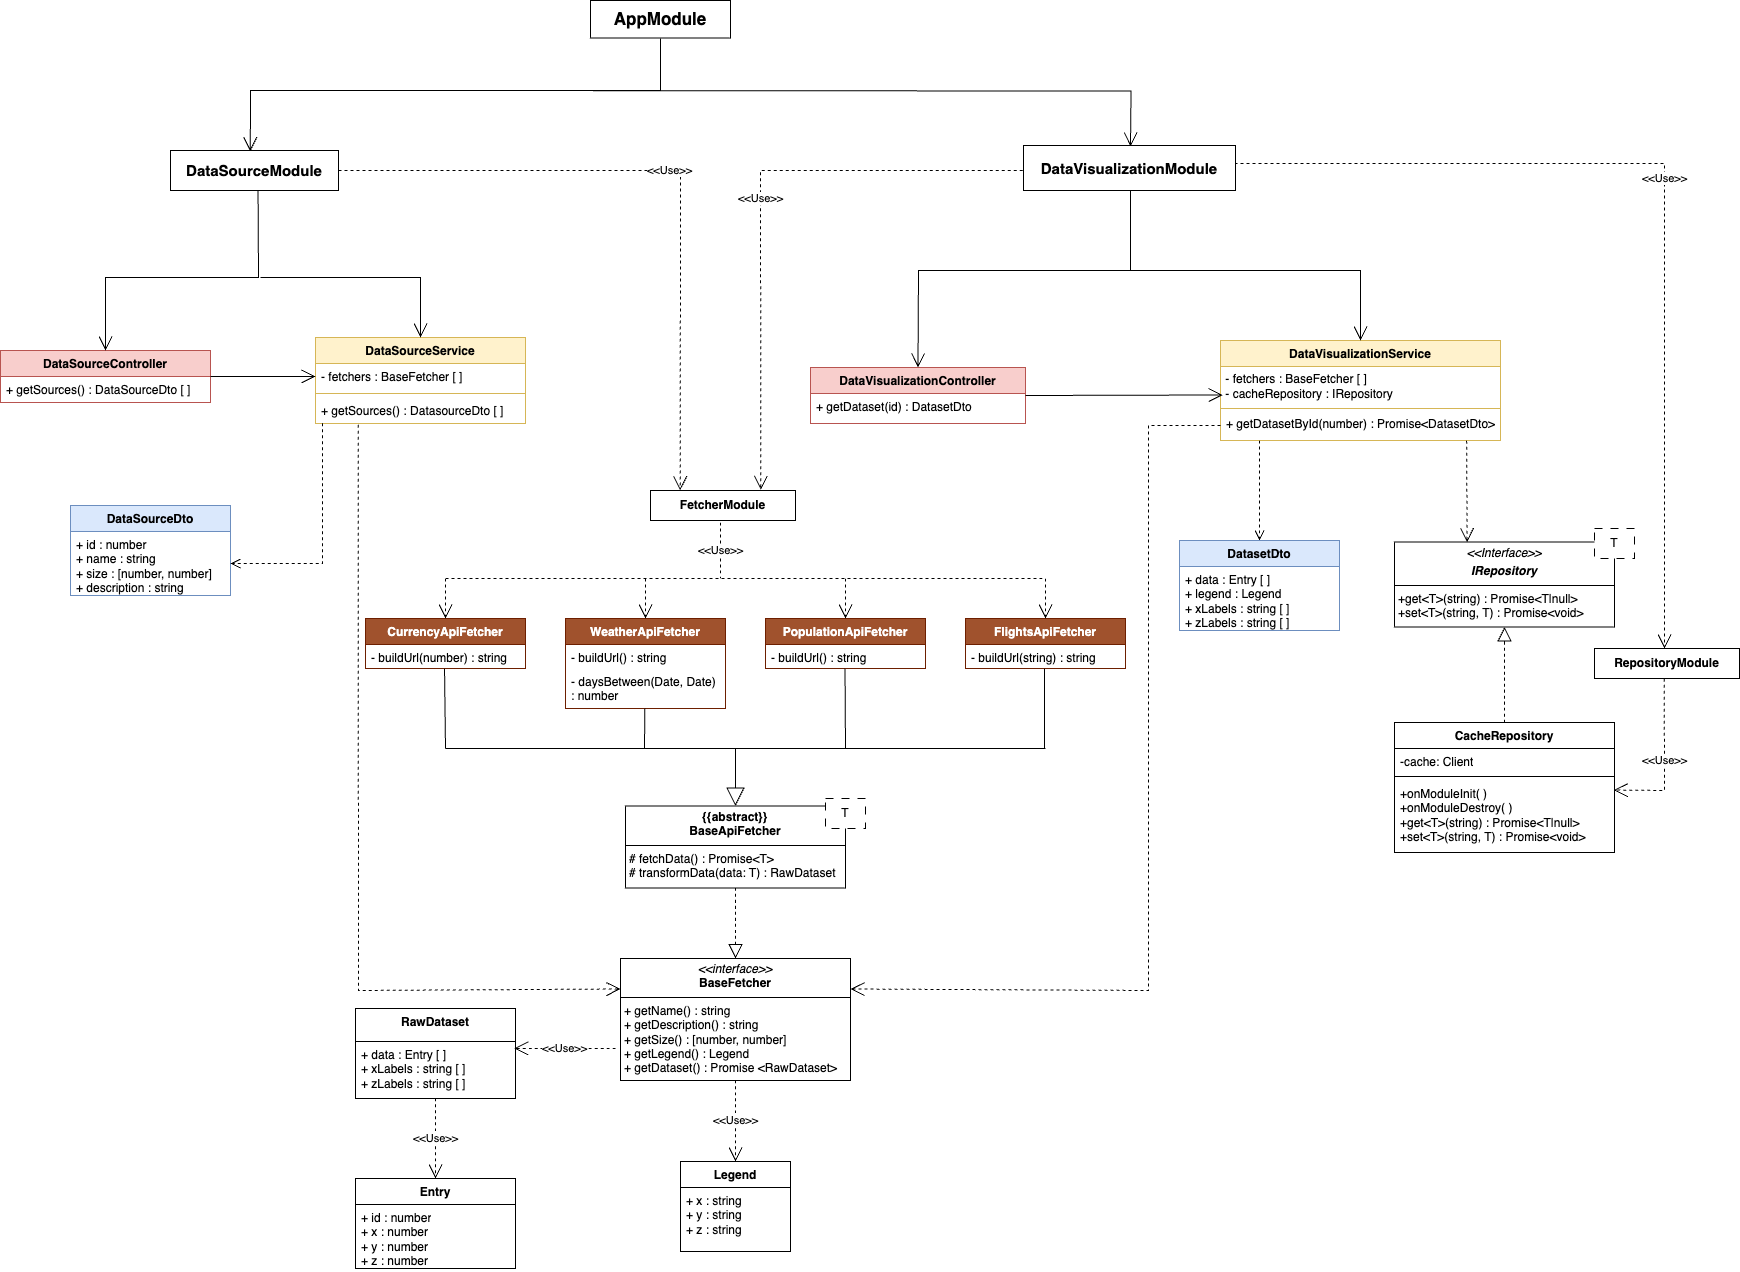
\includegraphics[scale = 0.29]{template/images/uml_back/BackendUML.png}
        \caption{Diagramma delle classi del backend}
    \end{center}     
    
\end{figure}

\subsubsection{Moduli}

L'architettura del sistema è suddivisa in moduli specializzati, ognuno dei quali gestisce una funzionalità o un'area logica specifica dell'applicazione. Questa organizzazione facilita l’indipendenza tra componenti, promuove il riuso del codice e permette di mantenere alta la qualità progettuale anche in presenza di modifiche o estensioni future.
Ogni modulo interagisce con il resto del sistema attraverso interfacce ben definite. Questo approccio, ispirato alla programmazione modulare.\\
In NestJS, ogni modulo è una classe annotata con un decoratore \texttt{@Module()} che organizza logicamente i componenti dell’applicazione, come controller e servizi. L’integrazione tra moduli avviene tramite il sistema di imports ed exports, che consente di condividere funzionalità in modo esplicito e controllato.

\paragraph{AppModule}

\begin{figure}[H] 
    \centering
    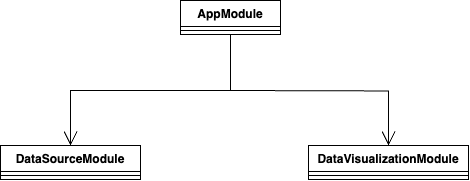
\includegraphics[scale = 0.5]{template/images/uml_back/AppModule.png}
    \caption{AppModule}
\end{figure}

L'AppModule rappresenta il punto di ingresso dell'applicazione e la sua funzione principale è quella di gestire e configurare i moduli principali. Questo modulo carica e configura i moduli \texttt{DataSourceModule} e \texttt{DataVisualizationModule}.

\paragraph{Moduli principali}
I moduli principali contengono la logica fondamentale dell'applicazione e sono responsabili della gestione e visualizzazione dei dati. I principali moduli dell'applicazione sono i seguenti:

\subparagraph{DataSourceModule}: 

\begin{figure}[H] 
    \centering
    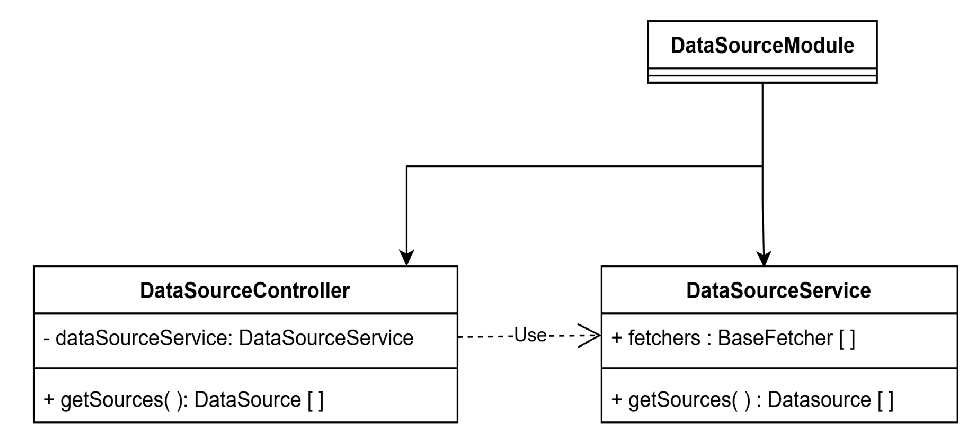
\includegraphics[scale = 0.55]{template/images/uml_back/DataSourceModule.png}
    \caption{DataSourceModule}
\end{figure}

Il \texttt{DataSourceModule} è responsabile della gestione delle metainformazioni relative alle fonti di dati disponibili nel sistema. Questo modulo incapsula la logica necessaria per raccogliere, organizzare e fornire informazioni descrittive sui dataset che l'applicazione può visualizzare.\\

\textbf{Responsabilità:}
\begin{itemize}
    \item Fornire un catalogo completo delle fonti dati disponibili;
    \item Recuperare metadati descrittivi per ciascuna fonte (nome, dimensione, descrizione);
    \item Esporre queste informazioni attraverso endpoint REST;
    \item Organizzare i metadati in strutture DTO coerenti per il consumo da parte del frontend.
\end{itemize}

\textbf{Componenti:}
\begin{itemize}
    \item \texttt{DataSourceController}: espone l'endpoint HTTP \texttt{GET /data-source} che restituisce la lista completa delle fonti dati disponibili. Gestisce le richieste in arrivo, le instrada al servizio appropriato e serializza le risposte.
    
    \item \texttt{DataSourceService}: implementa la logica di business per la raccolta dei metadati. Si interfaccia con i \texttt{fetcher} disponibili tramite l'interfaccia \texttt{BaseFetcher}, interrogando ciascuno per ottenere le informazioni descrittive necessarie. Questo servizio è responsabile della trasformazione dei dati grezzi in oggetti \texttt{DataSourceDto} ben strutturati.
    
    \item \texttt{DataSourceDto}: definisce la struttura dei dati trasferiti dal backend al frontend. Include:
    \begin{itemize}
        \item \texttt{id}: identificatore univoco della fonte dati;
        \item \texttt{name}: nome descrittivo della fonte;
        \item \texttt{size}: dimensione del dataset;
        \item \texttt{description}: descrizione dettagliata del contenuto della fonte.
    \end{itemize}
\end{itemize}

\textbf{Dipendenze:}
\begin{itemize}
    \item \texttt{FetcherModule}: fornisce al \texttt{DataSourceService} l'accesso ai fetchers tramite il token di iniezione \texttt{FETCHERS}. Ciò consente al servizio di utilizzare i fetcher disponibili senza preoccuparsi delle loro implementazioni specifiche o della loro creazione e configurazione diretta;
    \item \texttt{BaseFetcher}: interfaccia che definisce il contratto che ogni fetcher deve rispettare, inclusi i metodi per ottenere metadati descrittivi come \texttt{getName()}, \texttt{getDescription()} e \texttt{getSize()}.
\end{itemize}

\subparagraph{DataVisualizationModule}:

\begin{figure}[H] 
    \centering
    \includegraphics[scale = 0.5]{template/images/uml_back/DataVisModule.png}
    \caption{DataVisualizationModule}
\end{figure}

Il \texttt{DataVisualizationModule} gestisce la logica di recupero e formattazione dei dataset per la visualizzazione.\\

\textbf{Responsabilità:}
\begin{itemize}
    \item Recuperare il dataset completo dal fonte selezionato dall'utente tramite un ID specifico;
    \item Communicare con il cache per velocizzare il caricamento dei dati già richiesti in precedenza;
    \item Esporre un endpoint REST standardizzato per l'accesso ai dataset formattati.
\end{itemize}

\textbf{Componenti:}
\begin{itemize}
    \item \texttt{DataVisualizationController}: espone l'endpoint HTTP \texttt{GET /data-visualization/:id} che accetta l'ID numerico di un dataset e restituisce il dataset completo corrispondente;
    \item \texttt{DataVisualizationService}: implementa la logica per il recupero del dataset richiesto. Il servizio verifica la validità dell'ID, controlla la disponibilità dei dati nella cache e, se necessario, utilizza il fetcher appropriato per ottenere i dati dalla fonte esterna;
    \item \texttt{DatasetDto}: definisce la struttura dei dati restituiti al frontend, composta da:
    \begin{itemize}
        \item \texttt{rawData}: Dati grezzi recuperati dalla fonte esterna;
        \item \texttt{legend}: Informazioni sulla legenda del dataset.
    \end{itemize}
\end{itemize}

\subparagraph{Dipendenze:}

\begin{itemize}
    \item \texttt{FetcherModule}: Fornisce accesso all'array di \texttt{BaseFetcher} attraverso il token di iniezione \texttt{FETCHERS}. Questo permette al \texttt{DataVisualizationService} di recuperare i dati da diverse fonti in modo modulare, senza dipendere dalle implementazioni specifiche dei fetchers;
    \item \texttt{RepositoryModule}: Esporta il \texttt{CacheRepository} come implementazione concreta dell'interfaccia \texttt{IRepository}. Questo consente al \texttt{DataVisualizationService} di interagire con la cache tramite un'interfaccia astratta.
    \item \texttt{BaseFetcher}: Interfaccia che ogni fetcher implementa per fornire accesso standardizzato ai dati;
    \item \texttt{IRepository}: Interfaccia astratta per la gestione della cache. Definisce le operazioni fondamentali:
    \begin{itemize}
        \item \texttt{get(key: string)}: recupera un valore dalla cache;
        \item \texttt{set(key: string, value: T)}: salva un valore nella cache.
    \end{itemize}
    \item \texttt{CacheRepository}: Classe che implementa \texttt{IRepository}, fornendo la logica concreta per la lettura e scrittura nella cache. Registrata e esportata dal \texttt{RepositoryModule}.
\end{itemize}


\paragraph{Moduli di supporto}
I moduli di supporto forniscono funzionalità tecniche o infrastrutturali necessarie al funzionamento dell’applicazione.
Essi vengono progettati per essere riutilizzabili, indipendenti e incapsulati. Vengono esportati verso i moduli principali che ne fanno uso.
In questo progetto includono il \texttt{FetcherModule} e il \texttt{RepositoryModule}, che offrono rispettivamente l'accesso ai dati esterni e la logica di persistenza tramite cache.


\subparagraph{FetcherModule}:

\begin{figure}[H] 
    \centering
    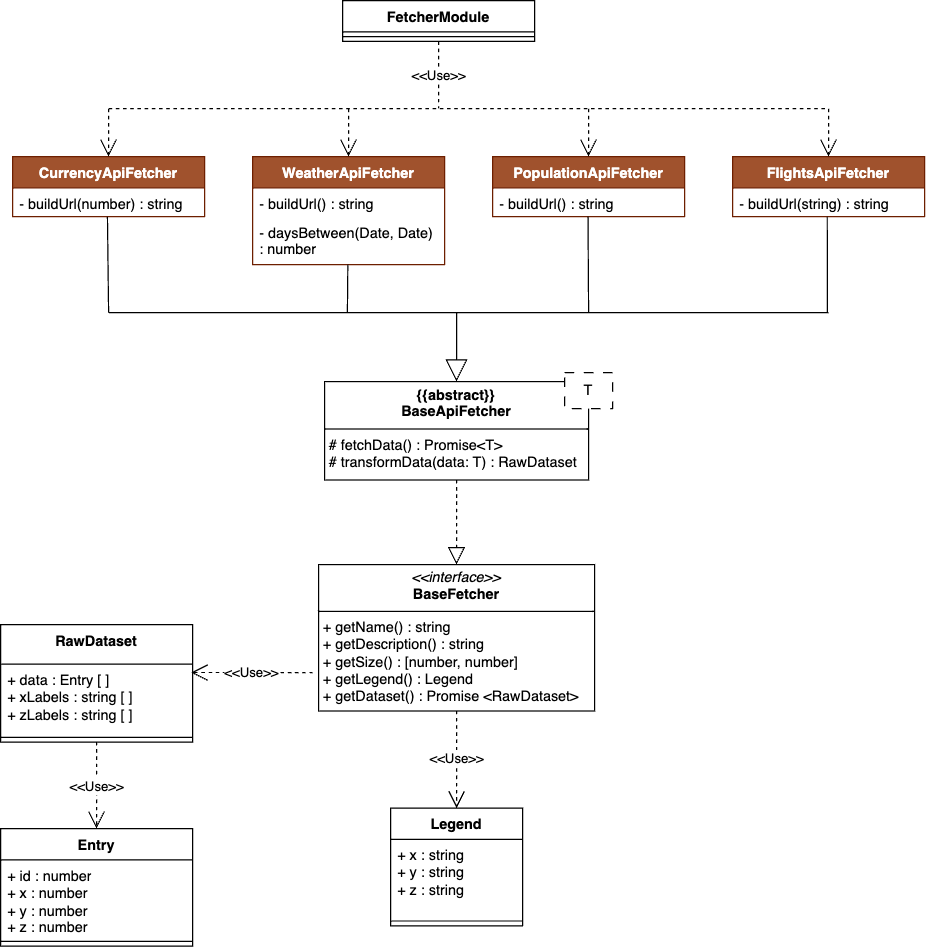
\includegraphics[scale = 0.5]{template/images/uml_back/FetcherModule.png}
    \caption{FetcherModule}
\end{figure}

Il \texttt{FetcherModule} incapsula tutti i componenti responsabili del recupero dei dati da fonti esterne, come API. Non contiene logica di business, ma espone un'interfaccia coerente per l’accesso ai dati, facilitando l’estensione e la manutenibilità del sistema.\\

\textbf{Responsabilità:}
\begin{itemize}
    \item Registrare e gestire i diversi \texttt{fetcher} che implementano l’interfaccia \texttt{BaseFetcher};
    \item Fornire un punto di accesso centralizzato e modulare alle fonti dati esterne.
\end{itemize}

\textbf{Struttura del modulo:}
\begin{itemize}
    \item \texttt{BaseFetcher}: interfaccia che definisce il contratto da rispettare per ogni \texttt{fetcher};
    \item \texttt{BaseApiFetcher}: classe astratta che offre una base comune per tutti i \texttt{fetcher} basati su API REST.
\end{itemize}

\textbf{Fetcher concreti:}
\begin{itemize}
    \item \texttt{WeatherApiFetcher}: recupera informazioni sulla temperatura media oraria per alcune grandi città europee, dal 01/01/2025 al 31/03/2025;
    \item \texttt{PopulationApiFetcher}: ottiene dataset contenente la popolazione totale di alcuni paesi dal 1974 al 2023;
    \item \texttt{FlightsApiFetcher}: fornisce il numero di partenze aeree da alcuni aeroporti internazionali nelle diverse fasce orarie in una giornata;
    \item \texttt{CurrencyApiFetcher}: restituisce tassi di cambio rispetto all'Euro campionati all'inizio di ogni anno dal 2005 al 2025.
\end{itemize}

\textbf{Integrazione con altri moduli:} \\
Il \texttt{FetcherModule} esporta il provider \texttt{FETCHERS}, che aggrega le istanze concrete dei \texttt{fetcher}. Questo consente agli altri moduli dell’applicazione di iniettarli facilmente, seguendo i principi dell’inversione delle dipendenze.

\subparagraph{RepositoryModule}:

\begin{figure}[H] 
    \centering
    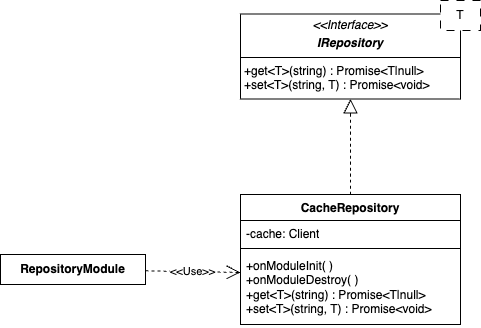
\includegraphics[scale = 0.5]{template/images/uml_back/RepositoryModule.png}
    \caption{RepositoryModule}
\end{figure}

Il \texttt{RepositoryModule} si occupa della persistenza temporanea dei dati applicativi, fornendo un’interfaccia coerente per la memorizzazione e il recupero di dati in cache. Questo modulo utilizza \texttt{Memcached} come sistema di caching distribuito, tramite il client \texttt{memjs}, fornendo così un meccanismo efficiente di persistenza temporanea per ottimizzare le performance dell'applicazione.\\

\textbf{Responsabilità:}
\begin{itemize}
    \item Fornire un meccanismo centrale per l’accesso ai dati temporanei;
    \item Isolare l’implementazione della cache dai servizi applicativi, attraverso l’uso di un’interfaccia.
\end{itemize}

\textbf{Struttura del modulo:}
\begin{itemize}
    \item \texttt{IRepository<T>}: interfaccia generica che definisce le operazioni base di salvataggio e lettura;
    \item \texttt{CacheRepository}: implementazione concreta che gestisce la connessione a Memcached e si occupa della serializzazione (conversione in stringa JSON) e deserializzazione dei dati per la loro corretta memorizzazione e recupero.
\end{itemize}

\textbf{Funzionalità del CacheRepository:}
\begin{itemize}
    \item Si connette al server Memcached all’avvio del modulo (\texttt{onModuleInit});
    \item Chiude la connessione in fase di distruzione del modulo (\texttt{onModuleDestroy});
    \item Metodo \texttt{get(key: string)}: recupera e deserializza il valore associato alla chiave specificata;
    \item Metodo \texttt{set(key: string, value: T)}: serializza e salva un valore con una chiave;
    \item Gestione robusta degli errori: i fallimenti di cache non interrompono il flusso del programma.
\end{itemize}

\textbf{Integrazione con altri moduli:} \\
Il modulo esporta la classe concreta \texttt{CacheRepository} come provider associato all'interfaccia \texttt{IRepository}. In questo modo, il \texttt{DataVisualizationService} dipende dall'interfaccia, mantiene un basso accoppiamento, mentre l'implementazione concreta viene risolta dal sistema di Dependency Injection.



\subsection{Pattern architetturale e Design pattern}

\subsubsection{Architettura Modulare (Modular Architecture)}
L’architettura del backend è progettata seguendo un approccio modulare, in cui ogni modulo rappresenta un'unità funzionale autonoma. Ciò consente di isolare le responsabilità, facilitando la manutenibilità e l'estensibilità del sistema. Ogni modulo è progettato per essere riutilizzabile e facilmente testabile, seguendo i principi della separazione delle preoccupazioni.

\subsubsection{Architettura a Strati (Layered Architecture)}
All'interno di ogni modulo, l'architettura a strati separa le diverse responsabilità: controller per la gestione delle richieste, servizi per la logica applicativa, e possibilmente DTO per la definizione dei dati scambiati. Questa separazione migliora la manutenibilità e la testabilità dell'applicazione.

\begin{itemize}  
  \item \textbf{Controller (Presentation Layer):} gestiscono le richieste in ingresso (es. HTTP) e costituiscono l'interfaccia tra il client e l'applicazione. Utilizzano decoratori come \texttt{@Controller} e \texttt{@Get} per definire le rotte e delegare la logica ai servizi sottostanti. Non contengono logica di business, ma si occupano di validare i dati tramite i DTO e restituire le risposte;
  
  \item \textbf{Service (Application Layer):} implementano la logica applicativa e gestiscono le operazioni necessarie per soddisfare le richieste. I servizi sono iniettati nei controller tramite il pattern di Dependency Injection e gestiscono la business logic dell'applicazione, interagendo con repository opppure fetcher;
  
  \item \textbf{DTO (Data Transfer Object):} definiscono i dati scambiati tra client e server, specificando le proprietà che devono essere validate e mappate. I DTO aiutano a garantire la coerenza dei dati e a documentare le API.
\end{itemize}

\subsubsection{Design Pattern Utilizzati}

In NestJS, abbiamo sfruttato diversi design pattern per semplificare la struttura e migliorare la manutenibilità del codice:

\begin{itemize}
  \item \textbf{Dependency Injection (DI):} Il pattern DI è utilizzato da NestJS per gestire le dipendenze tra i componenti. Grazie al decoratore \texttt{@Injectable()}, i servizi possono essere iniettati in altri servizi o controller. Questo approccio riduce il coupling e migliora la testabilità del sistema, evitando la creazione manuale delle istanze.

  \item \textbf{Decorator Pattern (con \texttt{@Controller} e \texttt{@Get}):} NestJS fa ampio uso del pattern decoratore, che permette di aggiungere comportamenti specifici ai componenti senza modificarne il codice. Il decoratore \texttt{@Controller} viene utilizzato per definire un controller, mentre \texttt{@Get} è impiegato per associare una rotta HTTP GET a un metodo del controller. Questi decoratori semplificano la gestione delle rotte e delle richieste HTTP.
  
  \item \textbf{Singleton:} Il pattern Singleton è applicato a livello di servizio, in quanto NestJS gestisce i provider come istanze uniche durante il ciclo di vita dell'applicazione. I servizi sono quindi condivisi tra i vari componenti, ottimizzando le risorse e riducendo il carico di creazione di nuove istanze.

  \item \textbf{Repository Pattern:} Utilizzato per astrarre la logica di accesso ai dati dalla logica di business, il Repository Pattern consente di gestire l'interazione con le fonti dati (come database o cache) in modo centralizzato. I repository vengono iniettati nei servizi, permettendo una gestione più flessibile dei dati.
\end{itemize}

